%%%%%%%%%%%%%%%%%%%%%%%%%%%%%%%%%%%%%%%%%
% baposter Portrait Poster
% LaTeX Template
% Version 1.0 (15/5/13)
%
% Created by:
% Brian Amberg (baposter@brian-amberg.de)
%
% This template has been downloaded from:
% http://www.LaTeXTemplates.com
%
% License:
% CC BY-NC-SA 3.0 (http://creativecommons.org/licenses/by-nc-sa/3.0/)

%----------------------------------------------------------------------------------------
%	PACKAGES AND OTHER DOCUMENT CONFIGURATIONS
%----------------------------------------------------------------------------------------

\documentclass[a0paper,portrait]{baposter}

\usepackage[font=small,labelfont=bf]{caption} % Required for specifying captions to tables and figures
\usepackage{booktabs} % Horizontal rules in tables
\usepackage{relsize} % Used for making text smaller in some places
\usepackage{subfig}
\usepackage{epstopdf}
\newcommand{\twoobjects}[2]{%
	\hbox{#1}\nointerlineskip\hbox{#2}%
}


\usepackage{float}

\graphicspath{{figures/}} % Directory in which figures are stored

\definecolor{bordercol}{RGB}{40,40,40} % Border color of content boxes
\definecolor{headercol1}{RGB}{186,215,230} % Background color for the header in the content boxes (left side)
\definecolor{headercol2}{RGB}{80,80,80} % Background color for the header in the content boxes (right side)
\definecolor{headerfontcol}{RGB}{0,0,0} % Text color for the header text in the content boxes
%\definecolor{boxcolor}{RGB}{186,215,230} % Background color for the content in the content boxes
\definecolor{boxcolor}{RGB}{255,255,255} % Background color for the content in the content boxes


\begin{document}

\background{ % Set the background to an image (background.pdf)
\begin{tikzpicture}[remember picture,overlay]
\draw (current page.north west)+(-2em,2em) node[anchor=north west]
{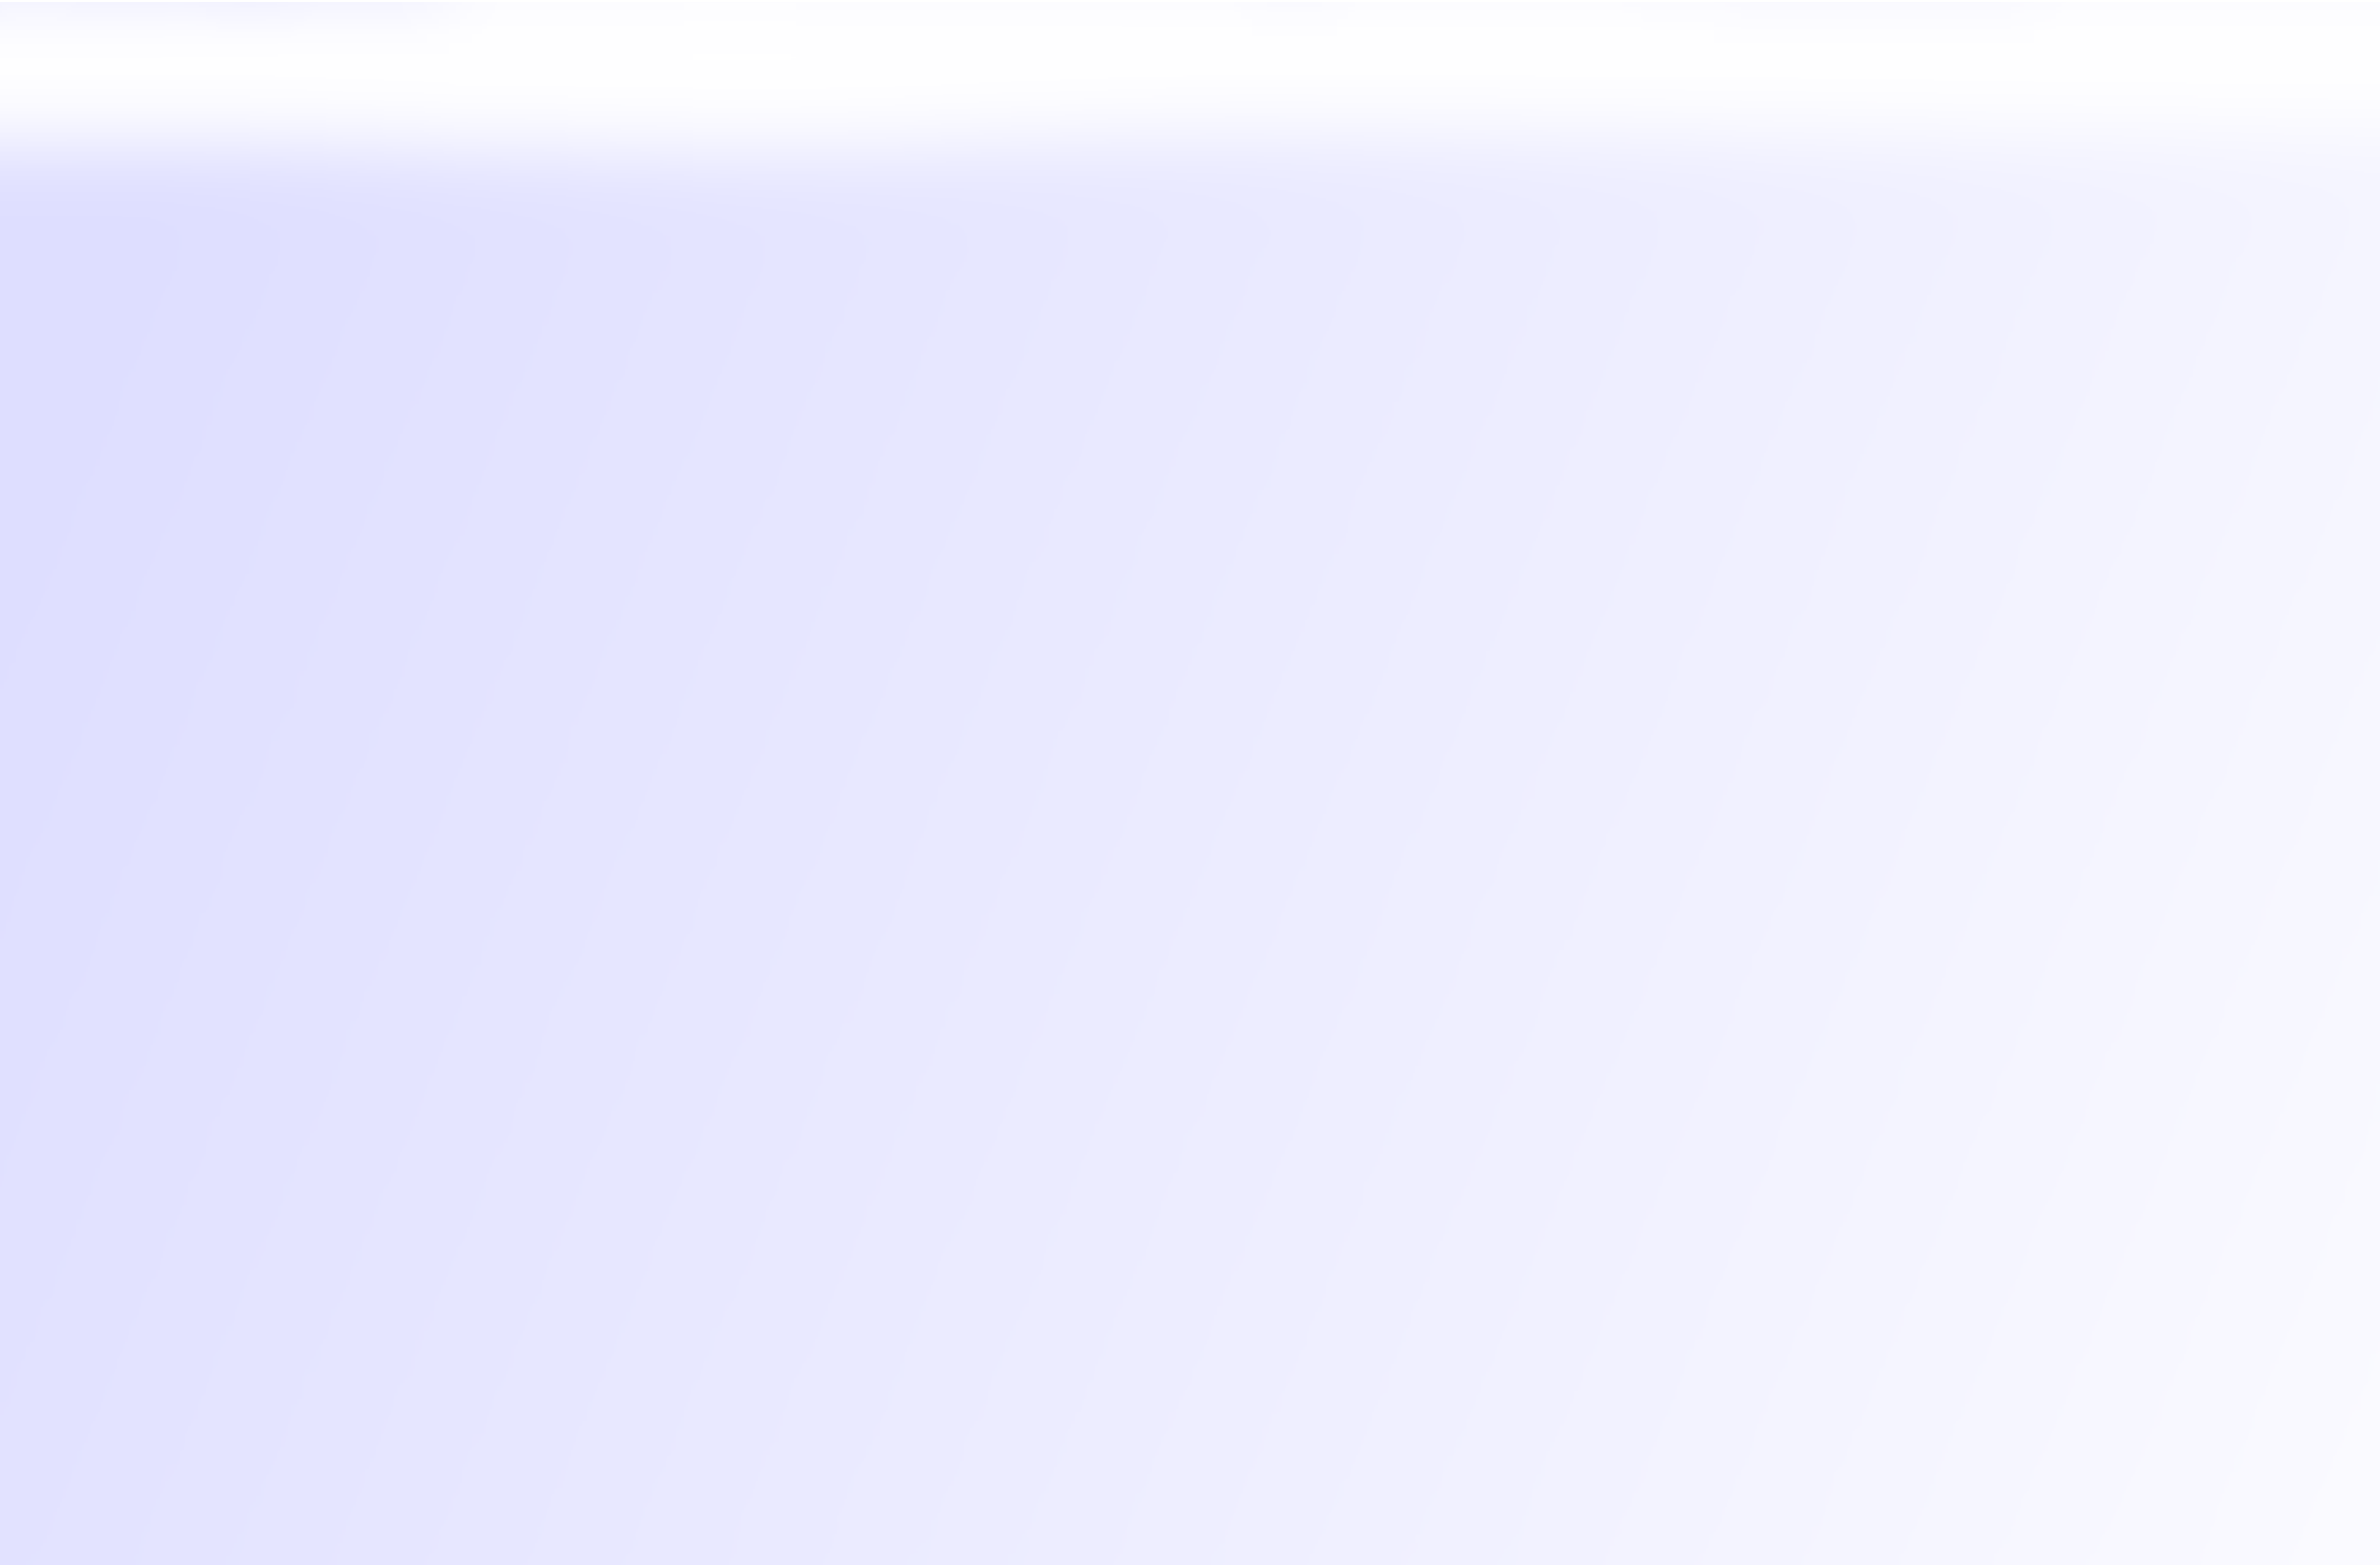
\includegraphics[height=1.1\textheight]{background}};
\end{tikzpicture}
}

\begin{poster}{
grid=false,
borderColor=bordercol, % Border color of content boxes
headerColorOne=headercol1, % Background color for the header in the content boxes (left side)
headerColorTwo=headercol2, % Background color for the header in the content boxes (right side)
headerFontColor=headerfontcol, % Text color for the header text in the content boxes
boxColorOne=boxcolor, % Background color for the content in the content boxes
headershape=roundedright, % Specify the rounded corner in the content box headers
headerfont=\Large\sf\bf, % Font modifiers for the text in the content box headers
textborder=rectangle,
background=user,
headerborder=open, % Change to closed for a line under the content box headers
boxshade=plain
}
{}
%
%----------------------------------------------------------------------------------------
%	TITLE AND AUTHOR NAME
%----------------------------------------------------------------------------------------
%
{\sf\bf AdVanScan: Computer Vision Team} % Poster title
{\vspace{1em} Bisbas G., Castiglione L., Kulon D., McMeel C., Ortiz J., Perez-Nieves N., Vink D.
\\ % Author names
} 
 {The logo on the left
	\begin{tabular}{lll}
		
\includegraphics[width=2cm]{royalmail} &
		
\includegraphics[width=4cm]{epsrc} &
		
\includegraphics[width=5cm]{imperial}
	\end{tabular}
}

%----------------------------------------------------------------------------------------
%	INTRODUCTION
%----------------------------------------------------------------------------------------

\headerbox{Abstract}{name=introduction,column=0,row=0}{
	
The goal of this work is to answer the question: \textbf{How full is the van?}

One of the volume estimation methods we considered was the use of a 3D camera. After comparing cameras, we chose the Intel RealSense, and took four pictures from different angles. The resulting point clouds were merged in MATLAB using an Iterative Closest Points (ICP) algorithm, and from the final point cloud a surface mesh was constructed. Using this, we obtained the value of the volume in the van by integration.

\begin{center}
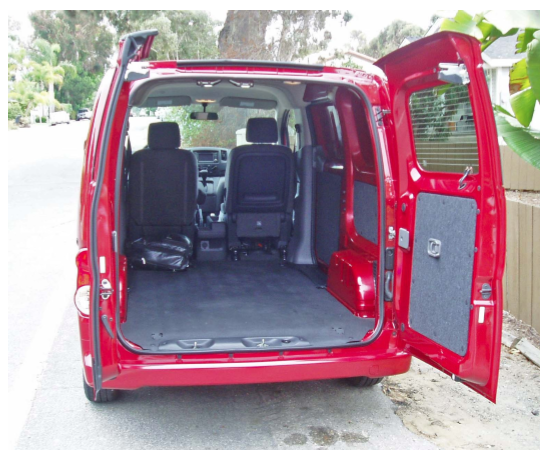
\includegraphics[width=0.8\linewidth]{van}
\end{center}
}

%----------------------------------------------------------------------------------------
%	MATERIALS AND METHODS
%----------------------------------------------------------------------------------------

\headerbox{Workflow outline}{name=methods,column=0,below=introduction}{
\begin{enumerate}
	\item Take pictures of the inside of the van from different angles.
	\item Extract point clouds from images.
	\item Merge point clouds via the ICP algorithm and fit a curve to this.
	\item Estimate the value of the volume using numerical integration.
\end{enumerate}

%------------------------------------------------


}

%----------------------------------------------------------------------------------------
%	CONCLUSION
%----------------------------------------------------------------------------------------

\headerbox{Challenges}{name=difficulties,column=0,below=methods}{

\begin{enumerate}
\item Large point cloud files (approx $20$Mb) slowed much of the procedure down and had to be simplified using well-known techniques.
\item Taking only one picture was found to have a lot of noise at the back of the van, so multiple pictures were taken in order to have a precise represenation.
\item The resulting point clouds would sometimes contain data from outside the van challenging the whole data processing. 
\item When measuring in a scenario where we know the volume occupied, some space is impossible to detect using pictures. This included space behind/between boxes, especially closer to the back of the van.
\end{enumerate}
}



%----------------------------------------------------------------------------------------
%	ACKNOWLEDGEMENTS
%----------------------------------------------------------------------------------------

\headerbox{Result Summary}{name=acknowledgements,column=0,below=difficulties, above=bottom}{
	\begin{itemize}
		\item Volume estimation in less than 45secs worst case.
		\item 5 to 7 \% error for ordered load and 9 to 11\% error for disordered
		\item No camera needed for every van.
		\item Total average error of almost 5\%, outliers excluded. 
	\end{itemize}
	

} 

%----------------------------------------------------------------------------------------
%	RESULTS 1
%----------------------------------------------------------------------------------------

\headerbox{Hardware Overview}{name=results1,span=2,column=1,row=0}{ % To reduce this block to 1 column width, remove 'span=2'

Discuss the pros/cons of various cameras and why we chose what we did.

We considered three different cameras before settling. The following table sums up some pros and cons of each.

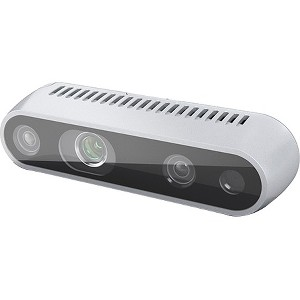
\includegraphics[width = 3.0cm]{Realsense1}
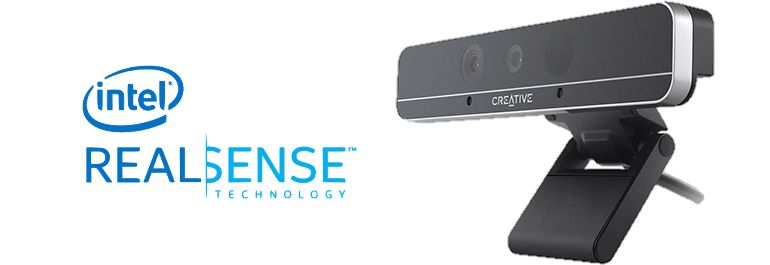
\includegraphics[width = 5.5cm]{intel2} \hspace{1cm}
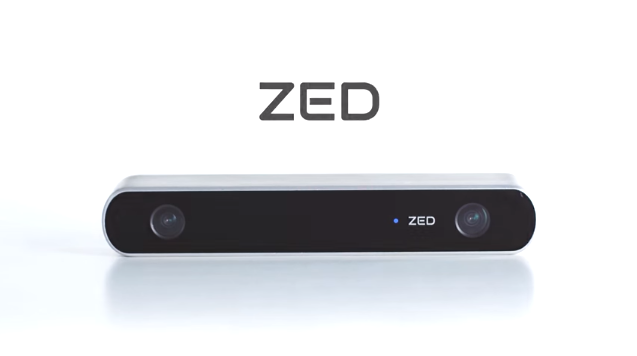
\includegraphics[width = 4.5cm]{ZED} \hspace{2cm}
\\ Intel Realsense SR$300$ is better for indoor locations due to infrared light while Zed Stereo Camera is better for outdoors. Our experiments using both of them, reassured this notion. After excluding the camera that didn't work, we settled on the Realsense $D435$ due to its superior price point and lack of dependence on environmental factors.
}
%----------------------------------------------------------------------------------------
%	RESULTS 2
%----------------------------------------------------------------------------------------

\headerbox{Workflow illustration}{name=results2,span=2,column=1,below=results1}{ % To reduce this block to 1 column width, remove 'span=2'
\vspace{0.2cm}
\begin{minipage}[h]{0.49\textwidth}
	\begin{center}
		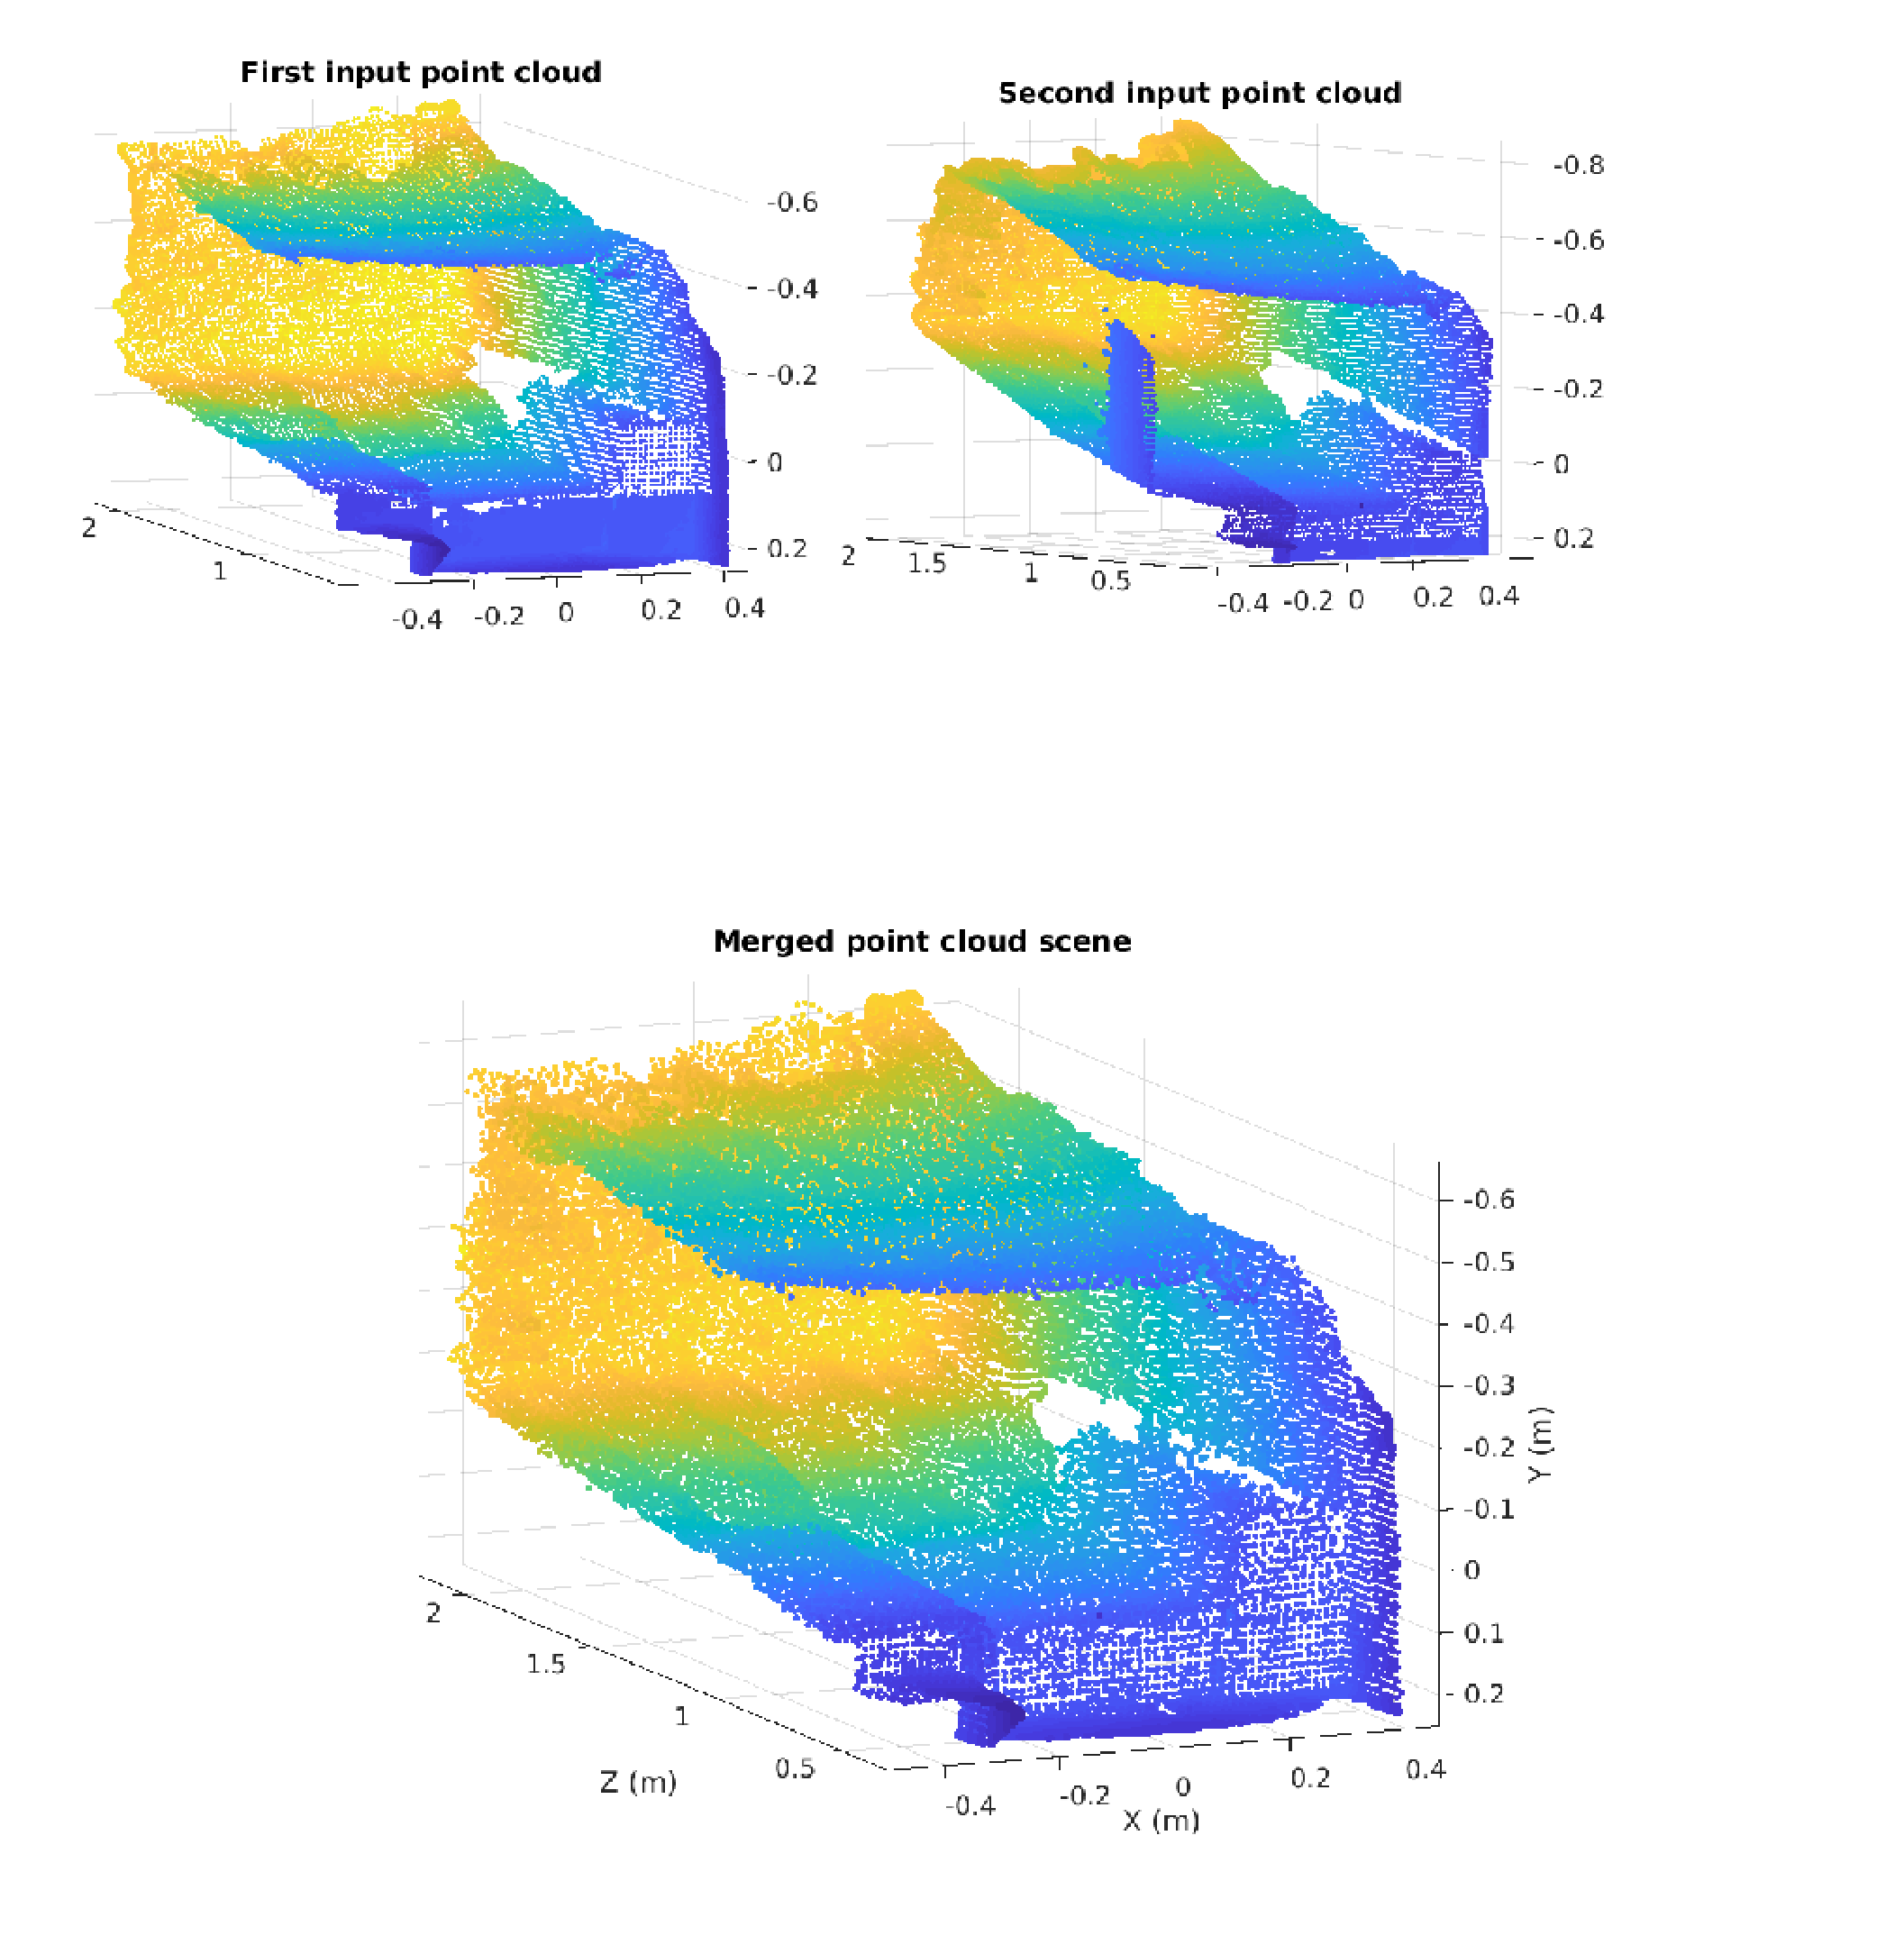
\includegraphics[width=0.99\linewidth]{merge_h.eps}
	\end{center}
	\captionof{figure}{Intermediate merged pointclouds (left) and final point cloud (right). Denoised and downsampled version of final point cloud (bottom).}
	\label{fig:2}
	
	\vspace{0.3cm}
	Fig \ref{fig:1} shows a point cloud after removing the outliers and applying curve fitting. Notice the presence of empty spaces as well as the noise, specially at the back of the van (in dark red ).
	\vspace{0.5cm}
	
	Using Mathworks' MatLab curve fitting toolbox we created a fit to the data using a Linear Interpolation and numerically evaluate the double integral.
	
\end{minipage}
%\hfill
\begin{minipage}[h]{0.49\textwidth}
	% Creating a reconstructed surface from the 3D camera images of the van consisted of 4 key steps: acquiring the correct images and their corresponding pointclouds, removing outliers, merging and downsampling the pointclouds, and interpolating between the points to reconstruct the surface.
	%\vspace{0.5cm}
	Four pictures of the inside of the van are captured from different angles. The point clouds obtained from the camera are noisy and contain several outliers as well as empty patches. \\
	
	In order to obtain an accurate reading, the outliers are removed by using a threshold and denoising the image. \\
	
	Fig.\ref{fig:2} shows the point clouds after the first merging (top) and the final result (bottom). The back of the van has been clearly smoothed out, and while some white space has remained a lot has been filled by the merging procedure.
	
	After this, the four images are downsampled and merged to obtain a final point cloud. The merging is done by using the well known Iterative Closest Points algorithm, thus not requiring to know the exact position at which the pictures were taken. (Independent of angle and direction)
	
	\begin{center}
		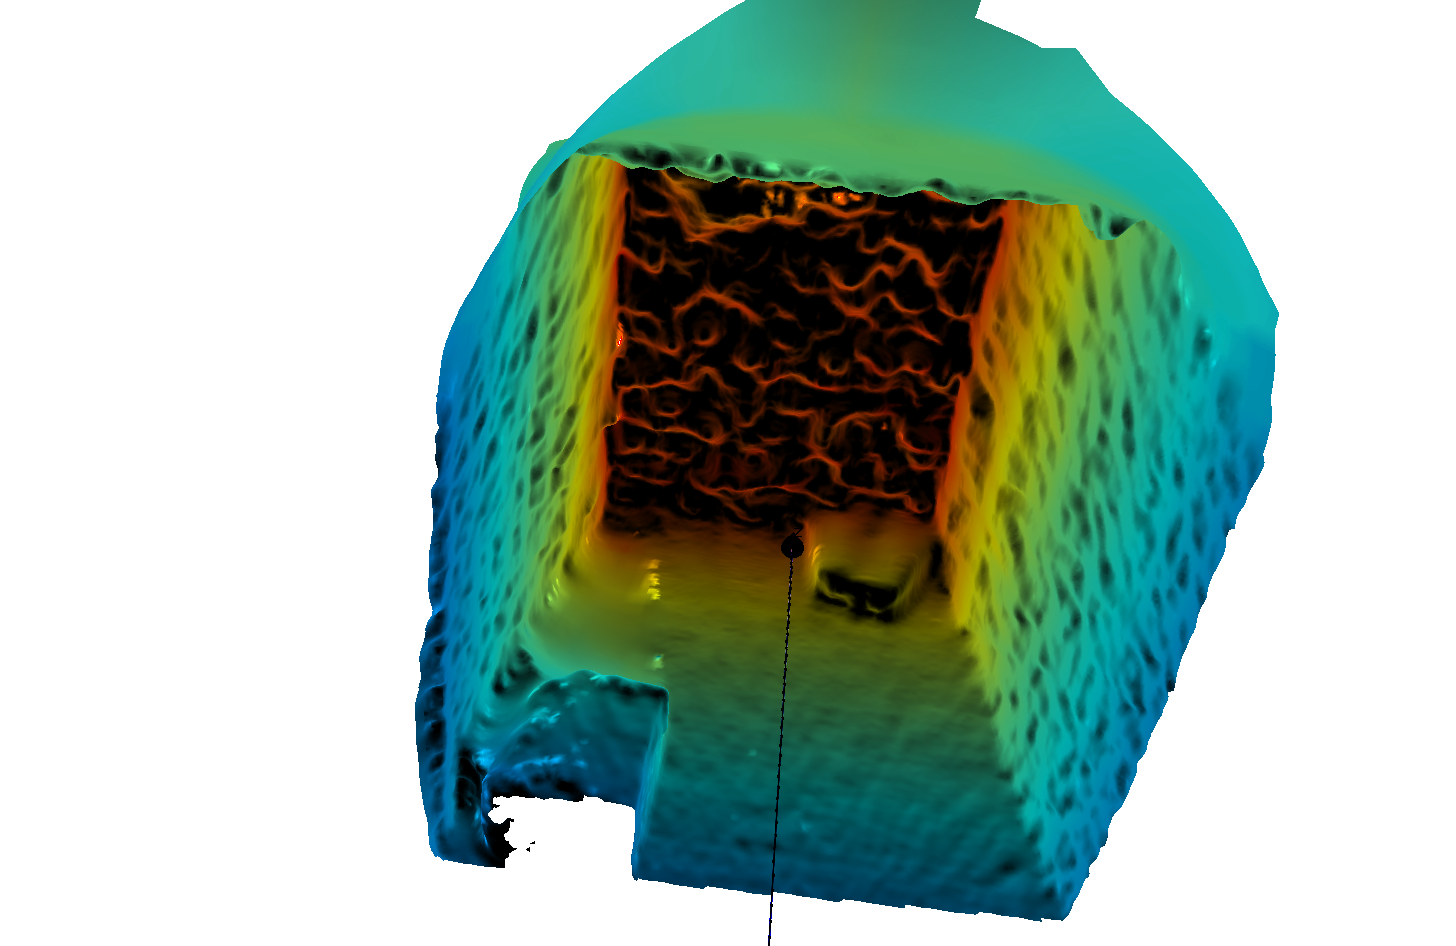
\includegraphics[width=0.8\linewidth]{van100.png}
		\captionof{figure}{Point cloud curve fitting}
		\label{fig:1}
	\end{center}
	
	%\vspace{10.5cm}
\end{minipage}%

}
\headerbox{References and acknowledgements}{name=references,span=2,column=1,below=results2, above=bottom}{
\begin{itemize}
	\item Johnson, a. E., \& Hebert, M. (1997). Surface registration by matching oriented points. Proceedings. International Conference on Recent Advances in 3-D Digital Imaging and Modeling (Cat. No.97TB100134).
	\item Besl, P., \& McKay, N. (1992). A Method for Registration of 3-D Shapes. Tpami.
	\item Kazhdan, M., \& Hoppe, H. (2013). Screened poisson surface reconstruction. ACM Transactions on Graphics, 32(3), 1–13.
	\item Amenta, N., Choi, S., \& Kolluri, R. K. (2001). The power crust. Proceedings of the Sixth ACM Symposium on Solid Modeling and Applications - SMA ’01, 249–266. 
	\item Kazhdan, M., Bolitho, M., \& Hoppe, H. (2006). Poisson Surface Reconstruction. Proceedings of the Symposium on Geometry Processing, 61–70. 
\end{itemize}
\small % Reduce the font size in this block
This project was proposed and supported by Royal Mail, EPSRC and Imperial College London. A special thanks to Jeremy Bradley and Ben Glocker for their support and advice.
}



%----------------------------------------------------------------------------------------

\end{poster}

\end{document}